\section{Probability Models and Axioms}
\subsection{Objectives}
\begin{enumerate}
	\item Sample Space 
	\item  Probability law 
		\begin{itemize}
		    \item Axioms 
		    \item  Properties that follow from axioms
		\end{itemize}
	\item Examples 
		\begin{itemize}
		    \item Discrete 
		    \item Continuous
		\end{itemize}
	\item Strengthen Countable additivity axioms and 
		discuss some mathematical subtleties
	\item  Interpretation of Probability
\end{enumerate}

\subsection{Probabilistic Model}
Probabilistic models consist of two elements 
\begin{enumerate}
    \item Possible Outcomes :- Sample Space
    \item  belief about likelihood of outcomes :- Probability Law
\end{enumerate}

\subsection{Sample Space}
\begin{definition*}
    List (set) of Possible outcomes. Denoted by $\Omega$. List must satisfy following .
    \begin{enumerate}
        \item Mutually Exclusive : if One outcome occur then Other Cannot occur 
	\item Collectively Exhaustive : outside of list can not occur
	\item At the right Granularity : to be explained in detail below 
    \end{enumerate}
\end{definition*}
\begin{figure}[H]
	\centering
	\def\svgwidth{0.3\columnwidth}
	\import{./images/}{sample_space.pdf_tex}
\end{figure}
Explanation on right granularity 

Consider a coin tossing experiment . 
There is obvious two outcomes Head and tail . So the sample space 
becomes 

$\{H,T\}$

Now Consider the same coin tossing experiment, but now while 
we toss the coin we also check weather if its raining or not (which
would be little silly thing to do) and the sample space becomes

\begin{center}
\{H and rain , H and no rain , T and rain , T and no rain\}
\end{center}

Now lets analyze both the sample space 

\begin{tabular}{l|l|p{7cm}}
	\toprule
Sample space properties	& \{H,T\} & \{ H and rain, H and no rain , T and rain , T and no rain\} \\
	\midrule
Mutually Exclusive  & \checkmark & \checkmark \\
Collectively Exhaustive  & \checkmark & \checkmark \\
At the right Granularity & \checkmark &  ? \\
	\bottomrule
\end{tabular}
here the second sample space may not represent right granularity,  because 
there is no reason to believe coin tossing may affect weather , or weather may
affect the outcome of coin tossing . 

But ultimately the question of which one is at right granularity depends upon the
question you want to consider Ex. if you have some  theory that weather may 
affect the behaviour of coin , Then second sample space may be considered legitimate.

\paragraph{Examples}

\begin{figure}[H]
  \centering
  \includegraphics[width=0.9\linewidth,page = 4]{../instructor/lectureslides01.pdf}
  \caption{fig: sample space example 6.0431x}
  \label{fig:Sample space example discrete}
\end{figure}

\begin{figure}[htb!]
  \centering
  \includegraphics[width=\linewidth,page = 5]{../instructor/lectureslides01.pdf}
  \caption{fig:samples space Continuous 6.0431x}
  \label{fig:}
\end{figure}

\subsection{Probability Axioms}
\begin{definition*}
    Event : Subset of Sample Space. Probability is assigned to events
\end{definition*}

\begin{figure}[H]
	\centering
	\def\svgwidth{0.7\columnwidth}
	\import{./images/}{events.pdf_tex}
\end{figure}

Axioms :	
    \begin{enumerate}

        \item Non negativity $P(A) \ge 0$
	\item Normalization $P(\Omega) = 1$ 
	\item Finite additivity 
		
		if $A \cap B = \phi$ then $P(A \cup B) = P(A) + P(B)$
		\begin{figure}[H]
			\centering
			\def\svgwidth{0.3\columnwidth}
			\import{./images/}{finite_additivity.pdf_tex}
		\end{figure}

		Explanation

		Think of $1$ pound of substance is smeared over entire 
		sample space $\Omega$ . Then amount of substance smeared
		over $A$  + amount of substance smeared over $B$ = 
		amount of substance smeared over $A \cup B$

    \end{enumerate}
    \textcolor{blue}{The above 3 axioms are sufficient to check 
    when deciding whether a mathematical model is Probabilistic }

\subsection{Properties of Probability}
following properties of Probability are consequence of above 
3 axioms. 
\begin{enumerate}

    \item $P(A) \le 1$ 
    \item $P(\Phi) = 0$
    \item $P(\{s_{1},s_{2}, ....... ,s_{k}\}) = P(\{s_{1}\}) + P(\{s_{2}\}) + ........... + P(\{s_{k}\})$
    \item if $A \subset B$ then $P(A) \le P(B)$
    \item for $A$ and $B$ not necessarily disjoint
	    $p(A \cup B) = P(A) + P(B) - P(A \cap B)$
    \item union bound $P(A \cup B) \le P(A) + P(B)$

\end{enumerate}

\subsection{Probability Calculation}
\begin{figure}[H]
  \centering
  \includegraphics[width=0.8\linewidth,page = 12]{../instructor/lectureslides01.pdf}
  \caption{probability calculation :Discrete}
  \label{fig:Probability calculation : Discrete}
\end{figure}

\begin{figure}[H]
  \centering
  \includegraphics[width=0.8\linewidth,page = 13]{../instructor/lectureslides01.pdf}
  \caption{probability calculation :Discrete}
  \label{fig:Discrete probabiliy law calculation : Discrete}
\end{figure}

\begin{figure}[H]
  \centering
  \includegraphics[width=0.8\linewidth,page = 14]{../instructor/lectureslides01.pdf}
  \caption{probability calculation :Continuous}
  \label{fig:Probability calculation : Discrete}
\end{figure}

Probability Calculation Steps : 
\begin{enumerate}

    \item Specify Sample Space
    \item Specify Probability Law TODO
    \item Identify the event of interest TODO
    \item Calculate ...

\end{enumerate}

\subsection{Countable additivity}

